\chapter[Convolution]{Convolution}
\label{ch:convolution}
\index{convolution in mathematics|(}
\section{Convolution in Mathematics}
\label{sec:convolution:mathematics}
\subsection{Definition}
\label{sec:convolution:mathematics:definitions}
\index{definition!convolution in mathematics}
Convolution is a mathematical operation on two functions to produce a result that reflects how one of the input functions is modified by the other input function.\newline
The convolution of functions $f(x)$ and $g(x)$ (denoted $f*g(x)$) is defined\cite{Bracewell2000}, for continuous functions $f$ and $g$, as\footnote{In order for the continuous convolution operator $f * g$ to be defined, both $f$ and $g$ must be integrable functions.}
\begin{equation}
(f * g) (t)\equiv\int_{-\infty}^{\infty} f(\tau) g(t-\tau)d\tau
\end{equation}
\begin{figure*}[h]
    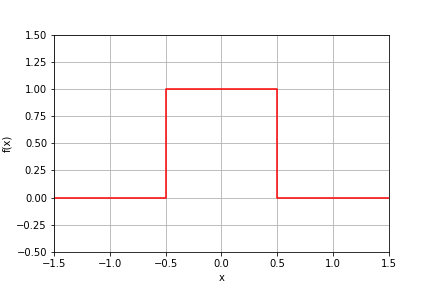
\includegraphics[width=.32\linewidth]{graphics/convolution/convolution_continuos_f_gebs.png}
    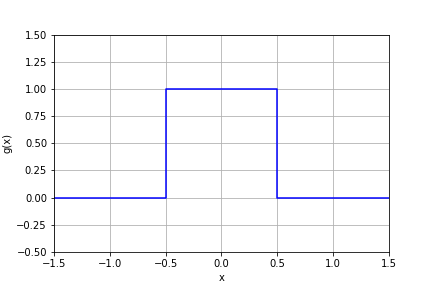
\includegraphics[width=.32\linewidth]{graphics/convolution/convolution_continuos_g_gebs.png}
    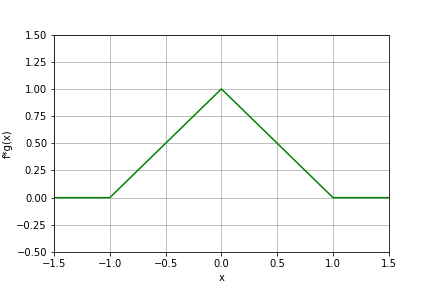
\includegraphics[width=.32\linewidth]{graphics/convolution/convolution_continuos_fg_gebs.png}
    \caption{These plots show two continuous functions ($f(x)$ and $g(x)$) and their convolution $f*g(x)$}.
    \label{fig:continuousconvolution}
\end{figure*}\FloatBarrier
and, for discrete functions $f(n)$ and $g(n)$, as
\begin{equation}
(f * g)(n)\equiv\sum_{m=-\infty}^{\infty}f(m) g(n-m)
\end{equation}
\begin{figure*}[h]
    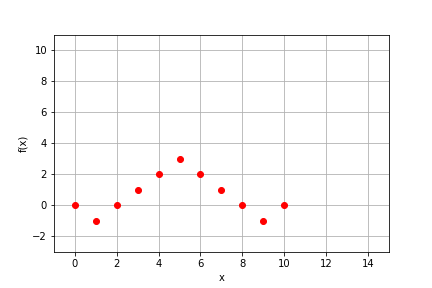
\includegraphics[width=.32\linewidth]{graphics/convolution/convolution_discrete_f_gebs.png}
    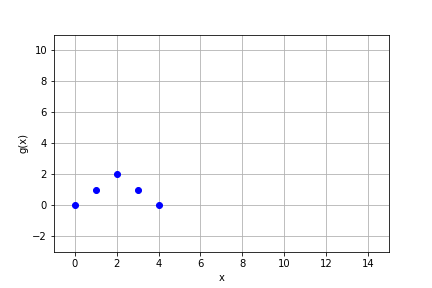
\includegraphics[width=.32\linewidth]{graphics/convolution/convolution_discrete_g_gebs.png}
    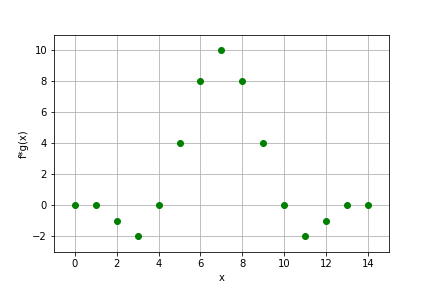
\includegraphics[width=.32\linewidth]{graphics/convolution/convolution_discrete_fg_gebs.png}
    \caption{These plots show two discrete functions ($f(n)$ and $g(n)$) and their convolution $f*g(n)$}.
    \label{fig:discreteconvolution}
\end{figure*}\FloatBarrier
\subsection{Properties}
\label{sec:convolution:mathematics:properties}
\index{properties!convolution in mathematics}
Since convolution is defined as a product of integrable functions on the linear space, the following algebraic properties are satisfied\cite{Bracewell2000}:\newline
\textbf{Commutativity}
\begin{equation}
(f * g)=(g * f)
\end{equation}
\textbf{Associativity}
\begin{equation}
(f * (g * h))=((f * g) * h)
\end{equation}
\textbf{Distributivity}
\begin{equation}
(f * (g + h))=(f * g) + (f * h)
\end{equation}
\textbf{Multiplication by a scalar value}
\begin{equation}
a (f * g) = (af) * g
\end{equation}
\textbf{Multiplicative identity}, where $\delta$ denotes the delta distribution 
\begin{equation}
f * \delta = f
\end{equation}
\textbf{Differentiation}
\begin{equation}
\frac{d}{dx}(f * g) = \frac{df}{dx} * g = f * \frac{dg}{dx}
\end{equation}
\textbf{Integration}
\begin{equation}
\int_{R^d} (f * g)(x)dx = \bigg(\int_{R^d} f(x)dx\bigg)\bigg(\int_{R^d} g(x)dx\bigg)
\end{equation}
\subsection{Applications}
\label{sec:convolution:mathematics:applications}
\index{applications!convolution in mathematics}
Listed below are some of the main applications of the convolution operator in various fields of knowledge\cite{Srivastava2013}:
\begin{itemize}
	\item \textbf{Image Processing} - Different operations are performed on images, in which the original image (larger matrix) and the filter to be applied (smaller matrix, also known as 2D kernel) are treated as 2-dimensional arrays. The kernel size and the values of its elements determine the effect on the original image
    \item \textbf{Signal Filtering} - Provided the filter function is the same as the impulse response function used in in signal filtering, the two operations are equivalent
    \item As a handy tool for \textbf{Polynomial Multiplication} - If we consider two polynomials being multiplied, we can use a convolution process to obtain the coefficients of the resulting polynomial
    \item \textbf{Audio Processing} - Reverberation is a desired effect in auditoriums, music halls, cinemas, and similar constructions. Convolution is used to digitally simulate reverberation in such structures, providing architects with information about the acoustic quality of a building prior to its construction
    \item \textbf{Artificial Intelligence} - Convolutional Neural Networks use convolution in one or more of its internal layers in order to process input data and enhance specific features.
    \item \textbf{Probability Theory} - The Probability Density Function (PDF) of the sum of two independent random variables can be obtained by the convolution of the PDFs of the two variables
\end{itemize}
\index{convolution in mathematics|)}
\index{convolutional neural networks|(}
\section{Convolution in Neural Networks}
\label{sec:convolution:convolutionalneuralnetworks}
\index{definition!convolutional neural networks}
\subsection{Definition}
\label{sec:convolution:convolutionalneuralnetworks:definition}
A Convolutional Neural Networks (CNNs) are a subclass of multi-layer neural networks in which some of its hidden layers are convolutional layers.\newline
Like most neural networks, CNNs can be trained using back-propagation algorithms and are mostly used to recognize visual patters with minimal or no preprocessing\cite{Lawrence1997A}.\newline
\index{origins and evolution!convolutional neural networks}
\subsection{Origins and Evolution}
\label{sec:convolution:convolutionalneuralnetworks:originsandevolution}
CNNs were initially developed as an attempt to replicate the processing of sight in living organisms.\newline
A seminal paper published in 1968\cite{Hubel1968} noted that two types of neurons took part in the process of identifying images: simple cells (responsible for the detection of straight edges and their orientation), and complex cells (with larger receptive fields, but not affected by the exact position of the edges in the input image).\newline
During the 1980s, CNNs evolved, followed by the introduction of Time Delay Neural Networks (TDNNs) in 1987\cite{Waibel1989}.\newline
In the early 1990s, CNNs were modified and used for medical image processing and for automatic detection of breast cancer in mammograms\cite{Zang1994}.\newline
In 1998 LeCun lead a team that created LeNet-5, a CNN used by banks to identify handwritten digits in checks.\newline
With the introduction of Graphic Processing Units (GPUs), training of CNNs was greatly improved, allowing for the implementation of efficient Deep Learning Neural Networks with impressive results in image processing and other applications \cite{Ciresan2013}.
\index{layers!convolutional neural networks}
\subsection{Layers}
\label{sec:convolution:convolutionalneuralnetworks:layers}
A typical CNN has sets of layers with specific functions, such as:
\begin{itemize}
    \item \textbf{Convolutional layer} - This is the main feature of a CNN.\newline
    In this layer, a set of filters (also known as kernels) is convoluted over the entire input data. The result of this operation (the activation map of the filter), extracts or enhances specific features in the input data that are passed to the following layers in the CNN.\newline
    Since the result of each convolution operation is affected by only a small part of the input data (due to the reduced size of the filter if compared to the size of the input data), this can be interpreted as each point of the activation map being affect by only a small subset of input points.
    \item \textbf{Pooling layer} - In this layer, simple operations are applied in order to reduce the size of the input data, such as maximum pooling or average pooling.\newline
    In 2x2 average pooling, for example, each result point the the average of 4 input points, reducing the size of the input field by a factor of 4.
    \item \textbf{Rectified Linear Unit (ReLU) layer} - This layer applies the $f(x) = max(0,x)$ activation function to its input, removing negative values from the input field.
    \item \textbf{Fully Connected layer} - In this layer, usually applied after several convolutional and pooling layers, neurons are connected to all activations in the previous layer, as in regular neural networks.
    \item \textbf{Loss layer} - This is the last layer in a typical CNN. In this layer, training is based on the divergence between the desired and predicted labels.
\end{itemize}
\index{training!convolutional neural networks}
\subsection{Training}
\label{sec:convolution:convolutionalneuralnetworks:training}
One important feature of CNNs is that, with the exception of the Loss layer, all other layers (Convolutional, Pooling, ReLU, and Fully Connected layers) can be trained using unsupervised training \cite{Arel2010}.\newline
Also, usually each layer or set of layers is trained individually, which also improves the speed and the overall result of the training.\newline
With the introduction of Graphic Processing Units (GPUs), speed of training and processing in the Convolutional layer has been greatly improved \cite{Steinkrau2005}
\index{applications!convolutional neural networks}
\subsection{Applications}
\label{sec:convolution:convolutionalneuralnetworks:applications}
CNNs are currently applied to a wide range of areas, such as \cite{Schmidhuber2015}:
\begin{itemize}
    \item \textbf{Image recognition and Video analysis} - Image Recognition Systems using CNNs are very efficient, specially if applied to facial recognition. Very good results have been obtained in challenges, and in the ImageNetNet tests performed almost as good as humans. If compared to image recognition, video analysis adds a level of complexity, since, in addition to the analysis of each frame, a time dimension needs to be added to the problem and convolution needs to be performed both on each image as well as on the time domain.
    \item \textbf{Game strategy} - A number of board games have been implements using CNNs, most notably Checkers, in Chess and in Go, the first time Artificial Intelligence beat an expert human player in this game.
    \item \textbf{Drug discovery} - In this area, CNNs are used to predict the behaviour of drug molecules and human proteins.
    \item \textbf{Natural language processing} - For NLP, CNNs are used extensively, including semantic parsing, search query retrieval, sentence modeling, classification, and prediction.
\end{itemize}
\clearpage
\index{convolutional neural networks|)}
\index{convolutional filters|(}
\section{Convolutional Filters}
\label{sec:convolution:convolutionalfilters}
\index{definition!convolutional filters}
\subsection{Definition}
\label{sec:convolution:convolutionalfilters:definition}
Convolutional filters (also known as kernels), when applied to image and video processing, are small square matrices with an odd number of rows and columns and used in the Convolutional layer of CNNs in order to detect or enhance specific features in the input image.\newline
The convolution operation performed by CNNs is a special two dimensional case of the discrete convolution operator.
\begin{equation}
R(m,n) = (K * I)(m,n)\equiv\sum_{s=-a}^{a}\sum_{t=-b}^{b}K(s,t)I(m-s,n-t)
\end{equation}
where $R(m,n)$ is the convoluted result at point $m,n$, $K$ is the kernel matrix being applied to the input matrix, $I$ is the input matrix, and $a$ and $b$ depend on the dimensions of the kernel used.
\index{common convolutional filters!convolutional filters}
\subsection{Common Convolutional Filters}
\label{sec:convolution:convolutionalfilters:commonconvolutionalfilters}
Convolutional filters can be defined to achieve a large range of effects in the input image.\newline
A small sample of possible kernels is provided below:\newline
\begin{itemize}
    \item \textbf{Identity} - This is the input image, without any convolution applied.
    $$
    \quad
    \begin{bmatrix} 
    0 & 0 & 0 \\
    0 & 1 & 0 \\
    0 & 0 & 0
    \end{bmatrix}
    $$
    \begin{center}
	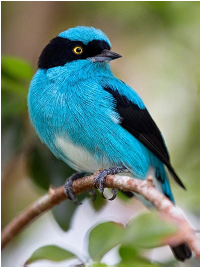
\includegraphics[width=1in]{graphics/convolution/Convolution_gebs_KernelIdentity.png}
    \end{center}
    \item \textbf{Gaussian blur}
    $$
    \frac{1}{16}
    \quad
    \begin{bmatrix} 
    1 & 2 & 1 \\
    2 & 4 & 2 \\
    1 & 2 & 1
    \end{bmatrix}
    $$
    \begin{center}
	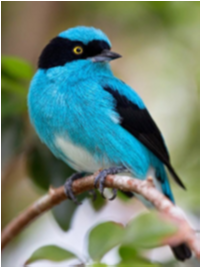
\includegraphics[width=1in]{graphics/convolution/Convolution_gebs_KernelGaussianBlur3x3.png}
    \end{center}
    \item \textbf{Box blur}
    $$
    \frac{1}{9}
    \quad
    \begin{bmatrix} 
    1 & 1 & 1 \\
    1 & 1 & 1 \\
    1 & 1 & 1
    \end{bmatrix}
    $$
    \begin{center}
	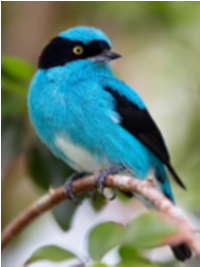
\includegraphics[width=1in]{graphics/convolution/Convolution_gebs_KernelBoxBlur.png}
    \end{center}
    \item \textbf{Unsharp}
    $$
    \frac{-1}{256}
    \quad
    \begin{bmatrix} 
    1 & 4 & 6 & 4 & 1 \\
    4 & 16 & 24 & 16 & 4 \\
    6 & 24 & -476 & 24 & 6 \\
    4 & 16 & 24 & 16 & 4 \\
    1 & 4 & 6 & 4 & 1
    \end{bmatrix}
    $$
    \begin{center}
	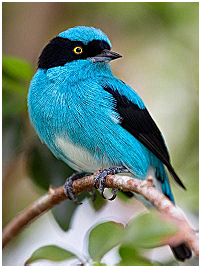
\includegraphics[width=1in]{graphics/convolution/Convolution_gebs_KernelUnsharp5x5.png}
    \end{center}
    \item \textbf{Sharpen}
    $$
    \quad
    \begin{bmatrix} 
    0 & -1 & 0 \\
    -1 & 5 & -1 \\
    0 & -1 & 0
    \end{bmatrix}
    $$
    \begin{center}
	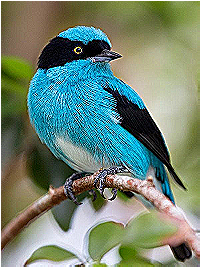
\includegraphics[width=1in]{graphics/convolution/Convolution_gebs_KernelSharpen.png}
    \end{center}
    \item \textbf{Edge detection}
    $$
    \quad
    \begin{bmatrix} 
    -1 & -1 & -1 \\
    -1 & 8 & -1 \\
    -1 & -1 & -1
    \end{bmatrix}
    $$
    \begin{center}
	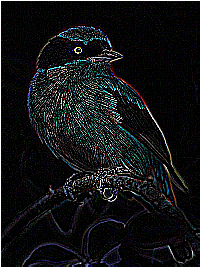
\includegraphics[width=1in]{graphics/convolution/Convolution_gebs_KernelEdgeDetection.png}
    \end{center}
\end{itemize}
\index{convolutional filters|)}
